\documentclass[handout]{beamer} 
\usetheme[numbering=none, progressbar=head]{metropolis} % \usetheme{PaloAlto}  \usecolortheme{owl}
\setbeamertemplate{itemize items}[circle]
\setbeamertemplate{section page}
{
    \begin{centering}
    \begin{beamercolorbox}[sep=12pt,center]{part title}
    \usebeamerfont{section title}\insertsection\par
    \end{beamercolorbox}
    \end{centering}
}
\setbeamertemplate{subsection page}
{
    \begin{centering}
    \begin{beamercolorbox}[sep=12pt,center]{part title}
    \usebeamerfont{subsection title}\insertsubsection\par
    \end{beamercolorbox}
    \end{centering}
}
% \usefonttheme[onlysmall]{structurebold}
% \usefonttheme[onlylarge]{structuresmallcapsserif}
% \useoutertheme{sidebar}
% \useinnertheme{circles}
% \insertframenumber/\inserttotalframenumber

%%%%%%%%%%%%%%
%  PACKAGES  %
%%%%%%%%%%%%%%
\usepackage[english]{babel}
\usepackage{hyperref}
\usepackage{amsmath}
\usepackage{mathrsfs}
\usepackage{multimedia} 

%%%%%%%%%%%
%  TITLE  %
%%%%%%%%%%%
\title{Autoencoders (Chapter 14)}
\author{Anna Lena Popkes, Pascal Wenker}% ()
\institute{Deep Learning Seminar \\ University of Bonn} 

\date{\today}
% \titlegraphic{\pgfuseimage{logo.png}}
% \logo{\includegraphics[height=0.5cm]{resources/logo.png}}

\begin{document}
\frame{\titlepage}
\begin{frame}[allowframebreaks]{Outline}
   % \frametitle{Outline}
   \begin{columns}
      \begin{column}{0.49\linewidth}
         \tableofcontents[sections=1-5, hideallsubsections]
      \end{column}\hfill%
      \begin{column}{0.49\linewidth}
          \tableofcontents[sections=6-10, hideallsubsections]
      \end{column}
   \end{columns}
\end{frame}

%%%%%%%%%%%%%%%%%%%%%%%
%  Table of Contents  %
%%%%%%%%%%%%%%%%%%%%%%%
% \begin{frame}[t]{Outline}
%    % \tableofcontents 
% \tableofcontents[ 
% section, 
% % hideallsubsections, 
% % sectionstyle=show/hide, 
% % subsectionstyle=show/shaded, 
% ] 
% \end{frame}
\begin{frame}[t]{Motivation}
    \begin{itemize}
   \item Which of the following number sequences do you find the easiest to memorize?
    \end{itemize}
       % \begin{itemize}
           A) 40, 27, 25, 36, 81, 57, 10, 73, 19 \\
           B) {\color<2,3,4>{red} 50, 25}, 76, 38, {\color<2,3,4>{blue}19, 58}, 29, 88, 44, 22, 11, 34, 17, 52, 26, 13 
\pause
\pause
   \begin{itemize}
       \item Two simple rules (Hailstone Sequence):
           \begin{enumerate}
               \item If the number is even, divide it by two: {\color{red} $x_{n+1} = x_n \div 2$}
               \item If the number is odd, triple it and add one: {\color{blue} $x_{n+1} = x_n \cdot 3 + 1$}
           \end{enumerate}
           \pause
   \end{itemize} 
           $\Rightarrow$ \textbf{Autoencoders are trained to discover and exploit patterns in the data}
\end{frame}

\setbeamercovered{transparent}
\section{Definition}
\begin{frame}[t]{Autoencoder - Task and Structure}
    \begin{figure}[h]
        \centering
        \includegraphics[scale=.5]{resources/figure14-1.jpg} 
        \caption{The general structure of an autoencoder.}
    \end{figure}
\begin{itemize}
    \pause
    \item Task: copy input to output
    \pause
    \item The network consists of two parts: 
        \begin{enumerate}
            \pause
            \item encoder function $\pmb{h} = f(\pmb{x})$
            \pause
            \item decoder that produces the reconstruction $\pmb{r} = g(\pmb{h})$
        \end{enumerate}
            \pause
        \item Loss function: $L(\pmb{x}, g(f(\pmb{x}))$
    \pause
            \item $\Rightarrow$ special type of a feed-forward network\\ 
\end{itemize}
\end{frame}


\begin{frame}[t]{Autoencoder - Goal}
   \begin{itemize}
       \pause
       \item Usually no interest in the output of the autoencoder
           \pause
       \item Don't copy the input perfectly to the output
           \pause
       \item Real goal: learn useful and efficient representations of the input data distribution\\
            \pause
            $\Rightarrow$ Restrict the autoencoder in some way\\
            \pause
            $\Rightarrow$ Example: Undercomplete autoencoders!
   \end{itemize} 
\end{frame}



\section{Undercomplete Autoencoders}
\begin{frame}[t]{Undercomplete Autoencoder - Definition}
    \begin{figure}[h]
        \centering
        \includegraphics[scale=.3]{resources/undercomplete_auto.png} 
        \caption{Structure of an Undercomplete Autoencoder}
    \end{figure}
    \begin{itemize}
        \pause
        \item Undercomplete $:=$ code dimension smaller than input dimension
            \pause
        \item Small code layer yields efficient representations and useful features  
        
    \end{itemize} 
\end{frame}

\begin{frame}[t]{Undercomplete Autoencoders - Capacity}
    \begin{itemize}
        \pause
        \item Linear decoder function + MSE $\Rightarrow$ undercomplete autoencoder learns to span same subspace as PCA
            \pause
        \item Nonlinear encoder and decoder $\Rightarrow$ undercomplete autoencoder can learn more powerful nonlinear generalizations than PCA!
            \pause
        \item Problem: if encoder and decoder are too powerful they learn only the copying task 
    \end{itemize}
\end{frame}


\begin{frame}[t]{Undercomplete Autoencoders - Problems}
    \begin{example}
        \begin{itemize}
            \item Very powerful nonlinear autoencoder with 1D code
        \pause
            \item Encoder: learns to map each training example $\pmb{x}^{(i)}$ to the code $i$
        \pause
            \item Decoder: learns to map these integer indices back to the values of specific training examples
        \end{itemize}
    \end{example}
\end{frame}

\section{Overcomplete Autoencoders}
\begin{frame}[t]{Overcomplete Autoencoder - Definition}
        \begin{figure}[h]
            \centering
            \includegraphics[width=0.9\linewidth]{resources/under_vs_over.png}
            \caption{Structure of undercomplete vs. overcomplete autoencoders}
        \end{figure}
        \pause
        \begin{definition}
        Overcomplete $:=$ code dimension larger than input dimension
        \end{definition}
\end{frame}

\begin{frame}[t]{Overcomplete Autoencoders - Problems}
    \begin{itemize}
        \item Problem: hidden dimension $\geq$ input dimension \\ 
            \pause
            $\Rightarrow$ even a linear autoencoder can copy the input to the output without learning anything useful
    \end{itemize} 
\begin{figure}[h]
    \centering
    \includegraphics[width=0.4\linewidth]{resources/overcomplete_auto_example.png}
    \caption{Overcomplete autoencoder that learned to copy its inputs to the coding layer and then to the output layer.} \end{figure}
\end{frame}

\section{Regularized Autoencoders}
\subsection{Motivation}
\begin{frame}[t]{Regularized Autoencoders - Motivation}
   \begin{itemize}
       \item Goal: choose code dimension and capacity of encoder/decoder based on the problem 
           \pause

        $\Rightarrow$ Find constraints that: 
           \begin{itemize}
               \item prevent the autoencoder from trivially copying the inputs directly to the outputs
                   \pause
               \item force it to learn efficient ways of representing the data
           \end{itemize}
   \end{itemize} 
\end{frame}

\begin{frame}[t]{Regularized Autoencoders - Definition}
   \begin{itemize}
       \item Regularized autoencoders modify the original loss function
           \pause
       \item The model is encouraged to have additional properties
           \pause
        \item Examples:
            \begin{enumerate}
                \item Sparse autoencoders: sparsity of the representation
                    \pause
                \item Denoising autoencoders: robustness to noise and outliers
                    \pause
                \item Contractive autoencoders: smallness of the derivative of the representation w.r.t. the input
                    \pause
            \end{enumerate}
            \pause
    \end{itemize} 
    $\Rightarrow$ 
    A regularized autoencoder can be overcomplete and nonlinear but still learn something useful about the data distribution!
\end{frame}


\subsection{Sparse Autoencoders}
\begin{frame}[t]{Regularized Autoencoders - 1. Sparse Autoencoders}
   \begin{itemize}
       \item A sparsity penalty on the code layer \pmb{h} is added to the reconstruction loss: $L(\pmb{x}, g(f(\pmb{x})) + \Omega{(\pmb{h})}$
           \pause
       \item $\Rightarrow$ Reduce number of active neurons
          \pause 
       \item Typically used to learn features for another task
           \pause
       \item The sparsity penalty can be interpreted in two ways:
           \begin{enumerate}
               \item Regularizer term for the copying task
                   \pause
               \item (Sparse autoencoder as approximation maximum likelihood training of a generative model that has latent variables)
           \end{enumerate}
   \end{itemize} 
\end{frame}

\subsection{Denoising Autoencoders}
\begin{frame}[t]{Regularized Autoencoders - 2. Denoising Autoencoders}
    \begin{itemize}
        \pause
    \item $L(\pmb{x}, \alert<3->{g(f(\tilde{\pmb{x}})})$ instead of $L(\pmb{x}, g(f(\pmb{x}))$   
        \pause
        \item Modified reconstruction error term
            \pause
        \begin{itemize}
        \item $\widetilde{\pmb{x}}$ is a copy of $\pmb{x}$ corrupted with some form of noise\\
        \end{itemize}
            \pause
            $\Rightarrow$ denoising autoencoders must learn to undo this corruption\\
            \pause
            $\Rightarrow$ $f$ and $g$ implicitly learn the structure of $p_{data}(\pmb{x})$
    \end{itemize}
\end{frame}


\subsection{Regularizing by Penalizing Derivatives}
\begin{frame}[t]{Regularized Autoencoders - 3. Penalizing Derivatives}
\begin{itemize}
    \pause
        \item We can also regularize by penalizing derivatives of the encoder function
            \pause
            % \item In this case, the penalty $\Omega$ takes a different form:\\
              \item $\Omega(\pmb{h},\pmb{x}) = \lambda \sum_i ||\alert<4->{\nabla_{\pmb{x}} h_i} ||^2$
               \pause 
               \pause
            \item This encourages the hidden representation to resist small changes in the input
                \pause
            \item Example: contractive autoencoders (CAE's)
\end{itemize}    
\end{frame}

\begin{frame}[t]{Recap}
   \begin{figure}[h]
       \centering
       \includegraphics[width=0.8\linewidth]{resources/flowchart_original_2.png}
       % \includegraphics[scale=.30]{resources/flowchart2.png}
   \end{figure} 
\end{frame}

\section{Representational Power, Layer Size and Depth}
\begin{frame}[t]{Representational Power, Layer Size and Depth}
    \begin{itemize}
\item Autoencoders often have only a single layer in the encoder and decoder
\pause
     \item Universal approximation theorem: a feed-forward network with a single hidden layer and enough hidden units can approximate any function to an arbitrary degree of accuracy\\
\pause
    $\Rightarrow$ An autoencoder with one hidden layer and enough hidden units can represent the identity function arbitrarily well
\pause
    \item Problem: we cannot enforce arbitrary constraints
\pause
    \item Solution: introduce an additional hidden layer in the encoder \\ $\Rightarrow$ model can approximate any mapping from input to code arbitrarily well

    \end{itemize}    
\end{frame}

\begin{frame}[t]{Representational Power, Layer Size and Depth}
    \begin{itemize}
        \item Depth can exponentially reduce the cost of representing some functions
\pause
        \item It also exponentially reduces the amount of needed training data
\pause
        \item Experimentally, deep autoencoders yield better compression than corresponding shallow or linear autoencoders
    \end{itemize}    
\end{frame}

\setbeamercovered{invisible}
\begin{frame}[t]{Questions}
    \begin{itemize}
        \item If an autoencoder perfectly reconstructs the inputs, is it necessarily a good autoencoder?\\ 
            \vspace{.3cm}
\pause
The fact that an autoencoder perfectly reconstructs its inputs does not necessarily mean that it is a good autoencoder; perhaps it is simply an overcomplete autoencoder that learned to copy its inputs to the codings layer and then to the outputs.
            \vspace{.3cm}
\pause
        \item What are undercomplete and overcomplete autoencoders?\\ 
            \vspace{.3cm}
            \pause    
An undercomplete autoencoder is one whose codings layer is smaller than the input and output layers. If it is larger, then it is an overcomplete autoencoder.
    \end{itemize}    
\end{frame}


\begin{frame}[t]{Questions}
    \begin{itemize}
        \item What is the main risk of an excessively undercomplete autoencoder? \\
            \vspace{.3cm}
            \pause
It may fail to reconstruct the inputs.
            \vspace{.3cm}
            \pause
        \item What about the main risk of an overcomplete autoencoder?\\
            \vspace{.3cm}
            \pause
It may just copy the inputs to the outputs, without learning any useful feature.
    \end{itemize}    
\end{frame}

\setbeamercovered{transparent}
\section{Stochastic Encoders and Decoders}
\begin{frame}[t]{Stochastic Encoders and Decoders}
   General strategy for designing output units and loss function:
\pause
   \begin{enumerate}
       \item Define output distribution $p(\pmb{y}\mid\pmb{x})$ 
\pause
           \item Minimize negative log-likelihood $-\log p(\pmb{y}\mid\pmb{x})$
   \end{enumerate}
\pause

   \vspace{0.3cm}
   \textbf{\underline{Autoencoders}}:
\pause
   \begin{itemize}
       \item $\pmb{x}$ is both input and target
\pause
       \item Given $\pmb{h}$, the decoder represents a conditional distribution $p_{decoder}(\pmb{x}\mid\pmb{h})$
\pause
       \item Loss function: $- \log p_{decoder}(\pmb{x}\mid\pmb{h})$
   \end{itemize}
\end{frame}


\begin{frame}[t]{Stochastic Encoders and Decoders}
    \begin{figure}[h]
        \centering
        \includegraphics[scale=.30]{resources/figure14-2.png}
        \caption{The structure of a stochastic autoencoder}
    \end{figure}
    \begin{itemize}
        \item We can further generalize the notion of an \textit{encoding function} $f(\pmb{x})$ to an \textit{encoding distribution} $p_{encoder}(\pmb{h} \mid \pmb{x})$
        \pause
        \item Any latent variable model $p_{model}(\pmb{h},\pmb{x})$ defines a stochastic encoder and decoder:\\
            $p_{encoder}(\pmb{h}\mid\pmb{x}) = p_{model}(\pmb{h}\mid\pmb{x})$\\
            \vspace{0.1cm}
            $p_{decoder}(\pmb{x}\mid\pmb{h}) = p_{model}(\pmb{x}\mid\pmb{h})$
    \end{itemize}
\end{frame}

\section{Denoising Autoencoders}
\subsection{Recap}
\begin{frame}[t]{Recap}
    \begin{itemize}
        \item Modified reconstruction error term
        \item $L(\pmb{x}, \alert{g(f(\tilde{\pmb{x}})})$ instead of $L(\pmb{x}, g(f(\pmb{x}))$   
            \begin{itemize}
            \item $\tilde{\pmb{x}}$ is a copy of $\pmb{x}$ corrupted with some form of noise\\
            \end{itemize}
            $\Rightarrow$ denoising autoencoders must learn to undo this corruption \\
            $\Rightarrow$ $f$ and $g$ implicitly learn the structure of $p_{data}(\pmb{x})$
    \end{itemize}
\end{frame}


\subsection{Training Procedure}
\begin{frame}[t]{Denoising Autoencoder -Training Procedure}
    \begin{columns}
        \column{0.3\linewidth}
        \begin{figure}[h]
            \centering
        \includegraphics[scale=.23]{resources/figure14-3.png}
            \caption{The computational graph of the cost function for a denoising autoencoder.}
        \end{figure}
        % \column{0.3\linewidth}
        % \includegraphics[scale=.23]{resources/figure14-3.png}
        \column{0.7\linewidth}
        \begin{itemize}
            \pause
            \item Introduce a corruption process $C( \pmb{\tilde{x}} \mid \pmb{x})$ 
            \pause
            \item The autoencoder then learns a \textit{reconstruction distribution} $p_{reconstruct}(\pmb{x}\mid\tilde{\pmb{x}} )$ as follows:\\
            \pause
                \begin{enumerate}
                    \item Sample a training example $\pmb{x}$ from the training data
            \pause
                    \item Sample a corrupted version $\pmb{\tilde{x}}$ from $C( \pmb{\tilde{x}} \mid \pmb{x})$
            \pause
                    \item Use $(\pmb{x},\pmb{\tilde{x}})$ as a training example for estimating the autoencoder reconstruction distribution $p_{reconstruct}(\pmb{x}\mid\pmb{\tilde{x}} ) = p_{decoder}(\pmb{x}\mid\pmb{h})$ 

                \end{enumerate}
        \end{itemize}
    \end{columns} 
\end{frame}

\begin{frame}[t]{Denoising Autoencoder - Training Procedure}
    \begin{figure}[h]
        \centering
        \includegraphics[width=1.0\linewidth]{resources/figure14-4.png}
        \caption{A denoising autoencoder is trained to map a corrupted data point $\tilde{\pmb{x}}$ back to
        the original data point $\pmb{x}$} 
    \end{figure}
\end{frame}



\section{Learning Manifolds with Autoencoders}
\begin{frame}[t]{Manifold Hypothesis}
    \begin{itemize}
        \item \textbf{Manifold hypothesis}: Data is concentrated around a low-dimensional \textit{manifold} or a small set of such manifolds
            \pause
        % \item In mathematics, a manifold is a topological space that locally resembles Euclidean space near each point 
        \item \textbf{Manifold}: Connected set of points that can be approximated well by considering only a small number of dimensions, embedded in a higher-dimensional space
    \end{itemize}    
\end{frame}

\begin{frame}[t]{Manifold Hypothesis}
    \begin{itemize}
        \item \textbf{Manifold hypothesis}: Data is concentrated around a low-dimensional \textit{manifold} or a small set of such manifolds
        % \item In mathematics, a manifold is a topological space that locally resembles Euclidean space near each point 
        \item \textbf{Manifold}: Connected set of points that can be approximated well by considering only a small number of dimensions, embedded in a higher-dimensional space
    \end{itemize}    
            \begin{figure}[h]
                \centering
                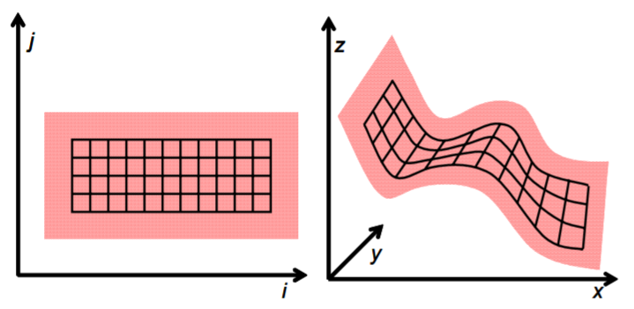
\includegraphics[scale=0.25]{resources/manifold.png}
                \caption{Data sampled from a distribution in a 2D space that is actually concentrated near a 1D manifold.}
            \end{figure}
\end{frame}


\begin{frame}[t]{Manifold Hypothesis}
        $\Rightarrow$ Autoencoders attempt to learn the structure of this manifold \\
            \vspace{.5cm}
            \begin{figure}[h]
                \centering
                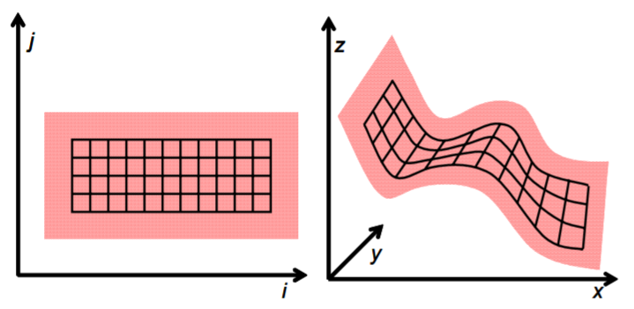
\includegraphics[scale=0.25]{resources/manifold.png}
                \caption{Data sampled from a distribution in a 2D space that is actually concentrated near a 1D manifold.}
            \end{figure}
\end{frame}



\begin{frame}[t]{Manifold Hypothesis - Evidence}
    \begin{itemize}
        \pause
        \item Manifold hypothesis does not always hold true
        \pause
        \item In the context of AI tasks (e.g. processing images, sound or text) at least approximately correct
            \pause
        \item Evidence given by two categories of observations
    \end{itemize} 
\end{frame}

\begin{frame}[t]{Manifold Hypothesis: Evidence 1}
    \begin{enumerate}
\item The probability distribution over images, text strings, and sounds that occur in real life is highly concentrated.
    \end{enumerate}
\begin{figure}[h]
    \centering
    \includegraphics[scale=0.15]{resources/figure5_12.jpg}
    \caption{Sampling images uniformly at random gives rise to noisy images. No faces. No cats.}
\end{figure}    
\end{frame}

\begin{frame}[t]{Manifold Hypothesis: Evidence 2}

\begin{itemize}
\item 
 Data points on a manifold are connected to each other via transformations
\end{itemize}
\pause
\begin{example}[Images]
   \begin{itemize}
    \item Dim or brighten the lights, move or rotate objects in the image, change the colors of objects, ...
   \end{itemize} 
\end{example}
\pause

\begin{itemize}
\item Likely, multiple manifolds are involved in most applications
    \pause
    \begin{itemize}
\item e.g. the manifold of images of human faces may not be connected to the manifold of images of cat faces
    \end{itemize}
\end{itemize}
\end{frame}


\begin{frame}[t]{Manifold Hypothesis - Recap}
    \begin{itemize}
    	\item Test
        $\Rightarrow$ Autoencoders attempt to learn the structure of this manifold \\
    \end{itemize}    
            \vspace{.5cm}
            \begin{figure}[h]
                \centering
                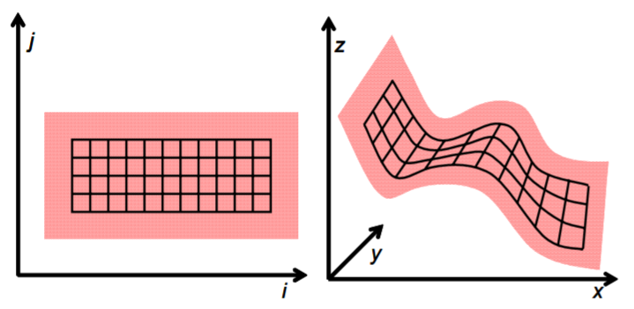
\includegraphics[scale=0.25]{resources/manifold.png}
                \caption{Data sampled from a distribution in a 2D space that is actually concentrated near a 1D manifold.}
            \end{figure}
\end{frame}

\subsection{Tangent planes}
\begin{frame}[t]{Tangent planes}
\begin{itemize}
    \pause
    \item An important characterization of a manifold is the set of its tangent planes
        \pause
    \item \textbf{Definition}: At a point $\pmb{x}$ on a $d$-dimensional manifold, the tangent plane is given by $d$ basis vectors that span the local directions of variation allowed on the manifold
    
\end{itemize} 
\end{frame}

\subsection{Tangent planes}
\begin{frame}[t]{Tangent planes}
\begin{itemize}
    \item An important characterization of a manifold is the set of its tangent planes
    \item \textbf{Definition}: At a point $\pmb{x}$ on a $d$-dimensional manifold, the tangent plane is given by $d$ basis vectors that span the local directions of variation allowed on the manifold
    
\end{itemize} 
        \begin{figure}[h]
            \centering
            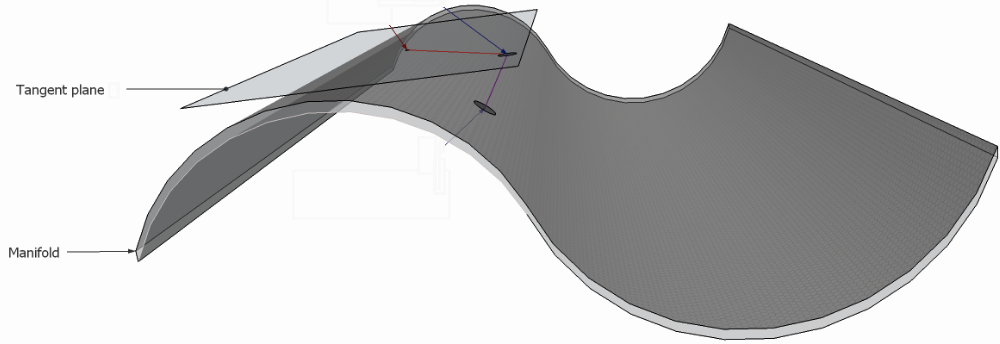
\includegraphics[width=0.8\linewidth]{resources/tangent_plane.png}
            \caption{A pictorial representation of the tangent space of a single point, \textbf{\textit{x}}, on a manifold.}
        \end{figure}
\end{frame}




\subsection{Autoencoder Training}
\begin{frame}[t]{Autoencoder Training}
    \begin{itemize}
        \item Autoencoder training procedures involve a compromise between two forces:
        \pause
            \begin{enumerate}
                \item Learning a representation $\pmb{h}$ of a training example $\pmb{x}$ such that $\pmb{x}$ can be approximately recovered from $\pmb{h}$ through a decoder
        \pause
                \item Satisfying the constraint or regularization penalty
            \end{enumerate}
        \pause
       \item Together, they force the hidden units to capture information about the structure of the data generating distribution
        \pause
    \item This yields representations that implicitly capture a local coordinate system for the manifold
   \end{itemize}
\end{frame}


\subsection{Comparison to other approaches}
\begin{frame}[t]{Comparison to other approaches}
    \begin{itemize}
        \item Common setting: a representation (embedding) for the points on the manifold is learned
        \pause
        \item Two different approaches
        \pause
            \begin{enumerate}
                \item Non-parametric methods: learn an embedding for each training example
        \pause
                \item Learning a more general mapping for \textit{any} point in the input space
            \end{enumerate}
        \pause
        \item Non-parametric approaches have problems with complicated manifolds\\
        \pause
            $\Rightarrow$ Motivates use of deep learning 
    \end{itemize}
\end{frame}


\section{Contractive Autoencoders}
\begin{frame}[t]{Contractive Autoencoders}
   \begin{itemize}
       \item Remember: contractive autoencoders are regularized autoencoders
        \pause
       \item Idea: extract only features that reflect variations found in the training set
        \pause
       \item CAE's add an explicit regularization term on the code $\pmb{h}$ to the reconstruction loss:\\
           \begin{center}
       $L(\pmb{x}, g(f(\pmb{x})) + \lambda \Vert \frac{\partial f(\pmb{x})}{\partial \pmb{x}} \Vert^2_F$ 
   \end{center}
        \pause
  $\Rightarrow$  Derivatives of the encoder function are encouraged to be small\\
        \pause
    $\Rightarrow$ Only a small number of input directions will have significant derivatives\\ 
        \pause
   $\Rightarrow$ The encoder function is encouraged to resist infinitesimal perturbations of the input
   \end{itemize} 
\end{frame}

\begin{frame}[t]{DAE's vs. CAE's}
    \begin{table}[h!]
        \centering
        \label{tab:}
        \begin{tabular}{p{5cm}|p{5cm}}
            \textbf{DAE} & \textbf{CAE}\\
            \hline
            \pause
            the \textit{decoder} function is trained to resist infinitesimal perturbations of the input & \pause the \textit{encoder} function is trained to resist infinitesimal pertubations of the input
        \end{tabular}
    \end{table}
\end{frame}

% \begin{frame}[t]{Problems of Contractive Autoencoders}
% \begin{frame}[t]{Problems of Contractive Autoencoders}
%     \item The regularization term is expensive to compute for deep autoencoders
%         \item The penalty term can 
        
% \end{itemize}
% \end{frame}



\begin{frame}[t]{DAE's vs. CAE's }
    \begin{itemize}
        \item Both the denoising and contractive autoencoder perform well
            \pause
        \item Advantage of denoising autoencoder: simpler to implement
            \pause
            \begin{itemize}
                \item Requires adding one or two lines of code to regular autoencoder
            \pause
                \item No need to compute Jacobian of hidden layer
            \end{itemize}
            \pause
        \item Advantage of contractive autoencoder: gradient is deterministic
            \pause
            \begin{itemize}
                \item Can use second order optimizers (conjugate gradient, LBFGS)
            \pause
                \item Might be more stable than denoising autoencoder, which uses a sampled gradient
            \end{itemize}
    \end{itemize}  
\end{frame}


\section{Applications of Autoencoders}
\begin{frame}[t]{Applications of Autoencoders}
    \begin{enumerate}
        \pause
        \item Dimensionality reduction
            \begin{itemize}
                \item Lower-dimensional representations can improve performance on many tasks (e.g. classification)
                \item Lower-dimensional models consume less memory and runtime
            \end{itemize}
\pause
\item Feature extraction
\pause
\item Unsupervised pretraining
            \pause
\item Generative models
    \end{enumerate}
\end{frame}

 
\setbeamercovered{invisible}
\begin{frame}[t]{Questions}
    \begin{itemize}
        \item What is the manifold hypothesis? What is its connection to autoencoders?\\
            \vspace{.3cm}
            \pause
        Manifold hypothesis: Data is concentrated around a low-dimensional \textit{manifold} or a small set of such manifolds
        Manifold. \\
        Autoencoders aim at learning the structure of the manifold(s).
    \end{itemize}    
\end{frame}


\begin{frame}[t]{Questions}
    \begin{itemize}
        \item What is special about the loss function of a denoising autoencoder?\\
            \vspace{.2cm}
            \pause
            Denoising autoencoders change the reconstruction error term of the cost function. Autoencoders traditionally minimize $L(\pmb{x}, g(f(\pmb{x})))$. The loss penalizes $g(f(\pmb{x}))$ for being dissimilar from $\pmb{x}$.\\
A DAE instead minimizes $L(\pmb{x}, g(f(\tilde{\pmb{x}})))$ where $\tilde{\pmb{x}}$ is a copy of \pmb{x} that has been corrupted with some form of noise. So instead of copying the input a DAE must learn to undo this corruption.
            \vspace{.3cm}
            \pause
        \item What are the main tasks autoencoders are used for?\\ 
            \pause
            \vspace{.2cm}
Feature extraction, unsupervised pretraining, dimensionality reduction, generative models
    \end{itemize}    
\end{frame}

%%%%%%%%%%%%%%
%  APPENDIX  %
%%%%%%%%%%%%%%
\appendix
\section{Appendix}


\begin{frame}[t]{Helpful Resources}
   \begin{itemize}
       \item YouTube video on contractive autoencoders: \url{https://www.youtube.com/watch?v=79sYlJ8Cvlc}
       \item YouTube video on denoising autoencoders: \url{https://www.youtube.com/watch?v=t2NQ_c5BFOc}
   \end{itemize} 
\end{frame}


\begin{frame}[t]{Sources}
If not listed below, all figures and definitions are taken from the Deep Learning book.
    \begin{itemize}
        \item Figure 10 (Tangent plane): \url{https://en.wikipedia.org/wiki/Tangent_space}
        \item Definition of Manifold: \url{https://en.wikipedia.org/wiki/Manifold}
\item DAE's versus CAE's slide: \url{https://www.youtube.com/watch?v=79sYlJ8Cvlc}
    \end{itemize}
\end{frame}

\begin{frame}[t]{Tangent planes - Example}
\begin{figure}[h]
    \centering
    \includegraphics[width=0.6\linewidth]{resources/figure14-6}
    \caption{An illustration of the concept of a tangent hyperplane}
    \label{fig:resources/figure14-6}
\end{figure}
\end{frame}
% End of document
\end{document}
